
\documentclass[12pt]{article}


\input{macros}

\usepackage{pgf}
\usepackage{tikz}

\begin{document}

\def\blattno{4}
\setcounter{uebno}{0}
\renewcommand{\datum}{}
\renewcommand{\beschreibung}{Seminar \blattno}




\newpage

\pagestyle{empty}
\setcounter{page}{1}
\pagestyle{plain}

\renewcommand{\solution}[1]{}





\renewcommand\thefigure{\arabic{figure}}    

\setcounter{figure}{0} 

\titel


\semex 
Figure \ref{fln-sem} represents a flow network $N=(D,c,s,t)$.

\begin{figure}[h!]
\begin{center}
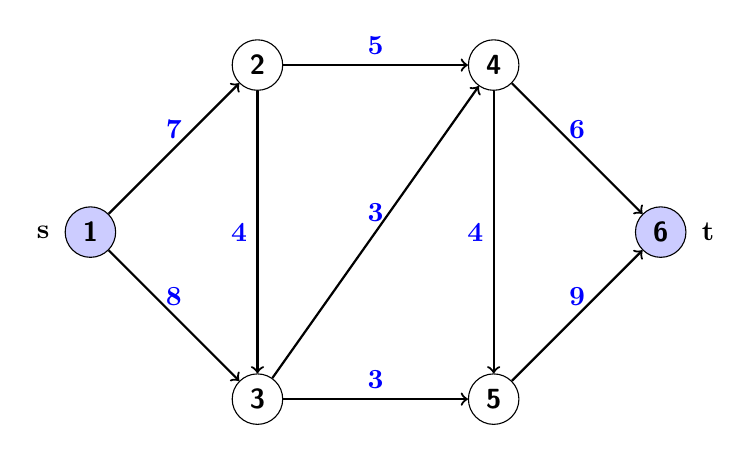
\begin{tikzpicture}
 [main node/.style={node distance=3cm, circle,fill=blue!20,draw,font=\sffamily\bfseries}, 
  normal node/.style={node distance=3cm, circle,fill=white!20,draw,font=\sffamily\bfseries}]
 
\node[main node] (1){1};
\node[normal node] (2)[above right of=1] {2};
\node[normal node] (3) [below right of=1] {3};
\node[normal node] (4) [right of=2] {4};
\node[normal node] (5) [right of=3] {5};
\node[main node] (6) [below right of=4] {6};
\node (s) [node distance=6mm, left of=1]{$\mathbf{s}$};
\node (t) [node distance=6mm, right of=6]{$\mathbf{t}$};
  
\path
  (1) edge [->, thick] node [above] {\textcolor{blue}{$\mathbf{7}$}} (2)
  (1) edge [->, thick] node [above] {\textcolor{blue}{$\mathbf{8}$}} (3)
  (2) edge [->, thick] node [left]      {\textcolor{blue}{$\mathbf{4}$}} (3) 
  (2) edge [->, thick] node [above] {\textcolor{blue}{$\mathbf{5}$}} (4)
  (3) edge [->, thick] node [above] {\textcolor{blue}{$\mathbf{3}$}} (4)
  (3) edge [->, thick] node [above] {\textcolor{blue}{$\mathbf{3}$}} (5) 
  (4) edge [->, thick] node [left]      {\textcolor{blue}{$\mathbf{4}$}} (5)
  (4) edge [->, thick] node [above] {\textcolor{blue}{$\mathbf{6}$}} (6) 
  (5) edge [->, thick] node [above] {\textcolor{blue}{$\mathbf{9}$}} (6);

\end{tikzpicture}
\caption{The flow network $N$}\label{fln-sem}
\end{center}
\end{figure}

Write the corresponding digraph $D$ and  
the capacity function $c$.
\solution{
We have that  $D=(V,A)$, where $V=\{1,2,3,4,5,6\}$ and 
\[A=\{(1,2),(1,3),(2,3), 
(2,4), (3,4),(3,5),(4,5), (4,6),(5,6)\}.\]

Furthermore, $c:A\to \Z_+$, $c(1,2)=7, c(1,3)=8, c(2,4)=5, c(2,3)=c(4,5)=4, 
c(3,4)=c(3,5)=3, c(4,6)=6, c(5,6)=9$.

}

\semex
Find vectors $b,d$ and a matrix $B$ such that
\[\max\{\text{value}(f) \mid f \text{ is an } s-t \text{ flow for } N\}=\max\{d^Tf \mid Bf\leq b\}.\]
\solution{Let $M$ be the incidence matrix of $D$ and  for every $i=1,\ldots, 6$, let us denote 
by $\mv_i$ the $i$-th line of $M$. Let $M_0$ be the matrix obtained from $M$ by deleting the lines 
$\mv_1$ and $\mv_6$. Thus, 
\bua
M=\bordermatrix{
~ & (1,2) & (1,3) & (2,3) & (2,4) & (3,4) & (3,5) & (4,5) & (4,6) & (5,6)  \cr
1 & -1 & -1 & 0 & 0 & 0 & 0 & 0 & 0 & 0\cr
2 & 1 & 0 & -1 &  -1 & 0 & 0 & 0 & 0 & 0\cr
3 & 0 & 1 & 1 & 0 & -1 & -1 & 0 & 0 & 0\cr
4 & 0 & 0 & 0 & 1 & 1 & 0 & -1 & -1 & 0\cr
5 & 0 & 0 & 0 & 0 & 0 & 1 & 1 & 0 & -1\cr
6 & 0 & 0 & 0 & 0 & 0 & 0 & 0 & 1 & 1\cr}, \\[2mm]
M_0=\bordermatrix{
~ & (1,2) & (1,3) & (2,3) & (2,4) & (3,4) & (3,5) & (4,5) & (4,6) & (5,6)  \cr
2 & 1 & 0 & -1 &  -1 & 0 & 0 & 0 & 0 & 0\cr
3 & 0 & 1 & 1 & 0 & -1 & -1 & 0 & 0 & 0\cr
4 & 0 & 0 & 0 & 1 & 1 & 0 & -1 & -1 & 0\cr
5 & 0 & 0 & 0 & 0 & 0 & 1 & 1 & 0 & -1\cr}.
\eua

Then (see Section 3.1.1 in the lecture notes),
\bua
\max\{\text{value}(f) \mid f \text{ is an } s-t \text{ flow}\} &=& \max\{\mv_6f \mid M_0 f=\ov, \ov\leq f\leq c\}\\
&=& \max\{d^Tf \mid Bf\leq b\},
\eua
where 
\[ d=\mv_6^T, \quad B=\begin{pmatrix} M_0\\ -M_0\\ I \\ -I \end{pmatrix}, 
\quad b =\begin{pmatrix} \ov \\ \ov \\  c\\ \ov \end{pmatrix}.\]
}

\semex
Figure \ref{fln-f-sem-1} represents an $s$-$t$ flow $f$ for the network $N$. 

\begin{figure}[h!]
\begin{center}
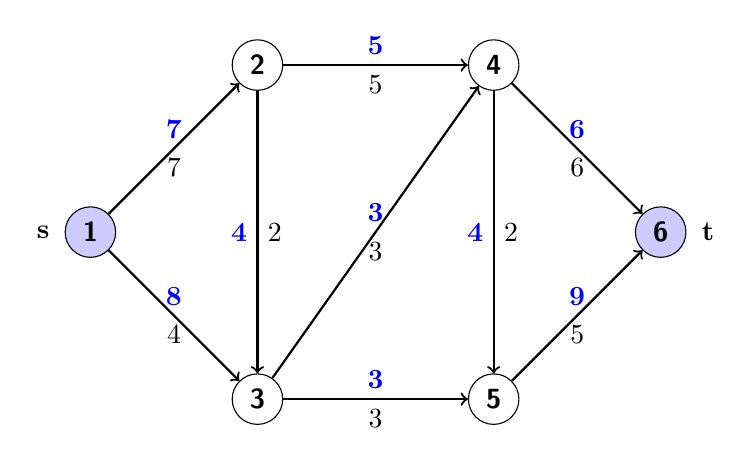
\begin{tikzpicture}
 [main node/.style={node distance=3cm, circle,fill=blue!20,draw,font=\sffamily\bfseries}, 
  normal node/.style={node distance=3cm, circle,fill=white!20,draw,font=\sffamily\bfseries}]
  
\node[main node] (1){1};
   \node[normal node] (2)[above right of=1] {2};
\node[normal node] (3) [below right of=1] {3};
 \node[normal node] (4) [right of=2] {4};
 \node[normal node] (5) [right of=3] {5};
  
  \node[main node] (6) [below right of=4] {6};

  \node (s) [node distance=6mm, left of=1]{$\mathbf{s}$};
  \node (t) [node distance=6mm, right of=6]{$\mathbf{t}$};  
   
\path
  (1) edge [->, thick] node [above] {\textcolor{blue}{$\mathbf{7}$}} node [below] {7} (2)
  (1) edge [->, thick] node [above] {\textcolor{blue}{$\mathbf{8}$}} node [below] {4} (3)
  (2) edge [->, thick] node [left] {\textcolor{blue}{$\mathbf{4}$}} node [right] {2} (3) 
  (2) edge [->, thick] node [above] {\textcolor{blue}{$\mathbf{5}$}} node [below] {5} (4)
  (3) edge [->, thick] node [above] {\textcolor{blue}{$\mathbf{3}$}} node [below] {3} (4)
  (3) edge [->, thick] node [above] {\textcolor{blue}{$\mathbf{3}$}} node [below] {3} (5) 
  (4) edge [->, thick] node [left] {\textcolor{blue}{$\mathbf{4}$}} node [right] {2} (5)
  (4) edge [->, thick] node [above] {\textcolor{blue}{$\mathbf{6}$}} node [below] {6} (6) 
  (5) edge [->, thick] node [above] {\textcolor{blue}{$\mathbf{9}$}} node [below] {5} (6);
       


\end{tikzpicture}
\caption{The flow network $N$ with the flow $f$}\label{fln-f-sem-1}
\end{center}
\end{figure}

\be
\item Verify that $f$ is an $s$-$t$ flow. What is the value of $f$?
\item Show that the set $\{(2,4), (3,4),(3,5)\}$ is an $s$-$t$ cut and compute its capacity.
\item Prove that $f$ is a maximum flow.

\ee
\solution{
\be
\item  $f:A\to \Z_+$ is defined by 
$f(1,2)=7, f(1,3)=4, f(2,3)=f(4,5)=2, f(3,4)=f(3,5)=3, f(2,4)=f(5,6)=5, 
f(4,6)=6$.
It is obvious that $0\leq f\leq c$. It remains to verify the flow conservation law
at every vertex $v\ne 1,6$:
\be
\item $v=2$. $in_f(2)=7, out_f(2)=2+5=7$
\item $v=3$. $in_f(3)=2+4=6, out_f(3)=3+3=6$
\item $v=4$. $in_f(4)=5+3=8, out_f(4)=2+6=8$
\item $v=5$. $in_f(5)=3+2=5, out_f(5)=5$.
\ee
We have that $\text{value}(f)=out_f(s)-in_f(s)=out_f(s)=7+4=11$.
\item Let $U=\{1,2,3\}$, hence $s\in U$, but $t\notin U$. We have that 
$\delta^{out}(U)=\{(2,4), (3,4),(3,5)\}$ and its capacity is $c(\delta^{out}(U))=5+3+3=11$.
\item Since $value(f)=c(\delta^{out}(U))$,  we can apply Corollary 3.0.9 to conclude that $f$ is a maximum flow. 
\ee
}

\semex
Let $N=(D,c,s,t)$ be a flow network and $f:A\to\R$ be an $s$-$t$ flow. Prove that 
the value of $f$ is equal to the net amount of flow entering $t$, that is  prove that 
$$\text{value}(f)=f(\delta^{in}(t))-f(\delta^{out}(t).$$
\solution{Applying Lemma 3.0.7 and the flow conservation law for $v\ne s,t$ we get that
\bua
0 & = & \text{excess}_f(V)= \sum_{v\in V} \text{excess}_f(v)=\sum_{v\in V\setminus\{s,t\}} \text{excess}_f(v)+
\text{excess}_f(s)+\text{excess}_f(t)\\
&=&\text{excess}_f(s)+\text{excess}_f(t).
\eua
Thus, $\text{value}(f)=-\text{excess}_f(s)=\text{excess}_f(t)=f(\delta^{in}(t))-f(\delta^{out}(t)$.
}


\semex
Let $N=(D,c,s,t)$ be a flow network with the property that all capacities are even (that is, $c(a)$ is even for every arc $a$ of $D$). Prove that the maximum value of a flow is even.
\solution{
Since all capacities are even, the capacity of every cut is even, hence the minimum capacity of a cut is even.
Apply the Max-Flow Min-Cut theorem to conclude that the maximum value of a flow is even.}



\end{document}


